\documentclass[11pt]{article}

\usepackage{amssymb}
\usepackage{xcolor}
\usepackage{verbatim}
\usepackage{multicol}
\usepackage{enumitem}
\usepackage{amsfonts}
\usepackage{amsmath}
\usepackage[utf8]{inputenc}
\usepackage[export]{adjustbox}  % for correct logo rendering
\usepackage{fancyhdr}  % for header/footer formatting
\usepackage{hyperref}  % for hyper-references
\usepackage{datetime}  % to update month in footer
\usepackage{array}  % more flexible tables
\usepackage[includeheadfoot,
            left=1in,
            right=1in,
            top=0.75in,
            bottom=0.75in,
            headheight=40pt]{geometry} % geometry needs to know headheight to correctly render the footer
\usepackage{tikz} % For drawing grid boxes

\definecolor{darkblue}{RGB}{0, 0, 139}
\definecolor{lightblue}{RGB}{173, 216, 230}

% desired format for footer
\newdateformat{monthyeardate}{%
  \monthname[\THEMONTH] \THEYEAR}

% set up header/footer
\pagestyle{fancy}
\fancyhf{}  % clear all headers/footers
\renewcommand{\headrulewidth}{0pt}  % remove header rule
\renewcommand{\footrulewidth}{0pt}  % remove footer rule

% set up header

\fancypagestyle{firstpage}{
    \fancyhead[L]{
    \vspace{0pt}
    \hspace{-8pt}
    
\includegraphics[width=0.1\textwidth]{docimgs/eth_logo_kurz_pos.png}\\
    \textbf{Swiss Federal Institute of Technology}\\
    \textbf{Zurich}\\
    %\textbf{ } \\
    
    }    

    \fancyhead[R]{
    \raggedleft
    %\vspace{20pt}
    
\includegraphics[width=0.13\textwidth]{docimgs/eth_ditet_logo_pos.png}\\
     \textbf{Dept. of Information Technology and} \\ \textbf{Electrical Engineering}  \\
     %\textbf{Chair for Mathematical Information} \\ \textbf{Information Science} \\

    }
}

% set up footer
\fancyfoot[L]{mdietz, ÜS 2}
\fancyfoot[C]{\thepage}
\fancyfoot[R]{\monthyeardate\today}

% set up section/subsection titles
\renewcommand{\thesection}{\arabic{section}}
\renewcommand{\thesubsection}{\arabic{subsection}}

% command used for simply emphasizing suggestions
\newcommand{\suggestion}[1]{{\itshape #1}}


\begin{document}
\thispagestyle{firstpage}

\setlength{\headheight}{1 \baselineskip}  % accomodate header
\setlength{\parindent}{0pt}  % remove initial paragraph indent
\setlength{\parskip}{\baselineskip}  % add skip between paragraphs

\vspace*{-5px}
\section*{Übungsstunde 2}

\section*{Themenüberblick}
\begin{itemize}
    \item \textbf{Hilberträume:}
    \item[] Inneres Produkt, Induzierte Norm, Orthogonalität, Pythagoras, Cauchy-Schwarz Ungleichung, Orthonormalsystem, $L^2$ als unendlich dimensionaler normierter Raum
    \item \textbf{Einführung Systeme und Systemeigenschaften:}
    \item[] Linearität, Nullraum und Bildraum, Stetigkeit
\end{itemize}

\section*{Aufgaben für diese Woche}
\vspace{-0.5cm}

\textbf{16}, 17, \textbf{18}, \textbf{19}, 20, \textbf{21}, 22, \textbf{23}, \textbf{24}\\
\vspace{-0.5cm}

Die \textbf{fettgedruckten} Übungen empfehle ich, weil sie wesentlich zu eurem Verständnis der Theorie beitragen und/oder sehr prüfungsrelevant sind.

\vfill \null
\pagebreak

\section*{Hilberträume}

\vspace*{-0.5cm}
\textbf{Definition:} Ein Hilbertraum ist ein linearer Raum, der mit einem inneren Produkt ausgestattet und vollständig bezüglich der durch das innere Produkt induzierten Norm ist.

\vspace*{-0.5cm}
\subsubsection*{Was verstehnt man unter Vollständigkeit?}
\vspace*{-0.5cm}
Vollständigkeit in einem Hilbertraum bedeutet, dass jede Cauchy-Folge in diesem Raum zu einem Element innerhalb des Raums konvergiert. Eine Cauchy-Folge ist eine Folge, bei der die Glieder im Verlauf der Folge beliebig nah aneinander liegen. In einem vollständigen Raum hat eine solche Folge immer einen Grenzwert, der ebenfalls zum Raum gehört. In einem Raum mit Löchern könnte es eine Cauchy-Folge geben, deren Punkte sich immer weiter an den Rand des Lochs annähern, aber egal wie weit man fortfährt, erreicht die Folge nie wirklich einen Punkt im Inneren des Lochs, weil dieser Punkt im Raum fehlt. Somit konvergiert die Folge zu keinem Element im Raum, was die Vollständigkeit verletzt. Intuitiv kann man sich also ein vollständigen Raum so vorstellen, dass er keine Löcher haben darf.

\begin{center}
    \begin{multicols}{2}
        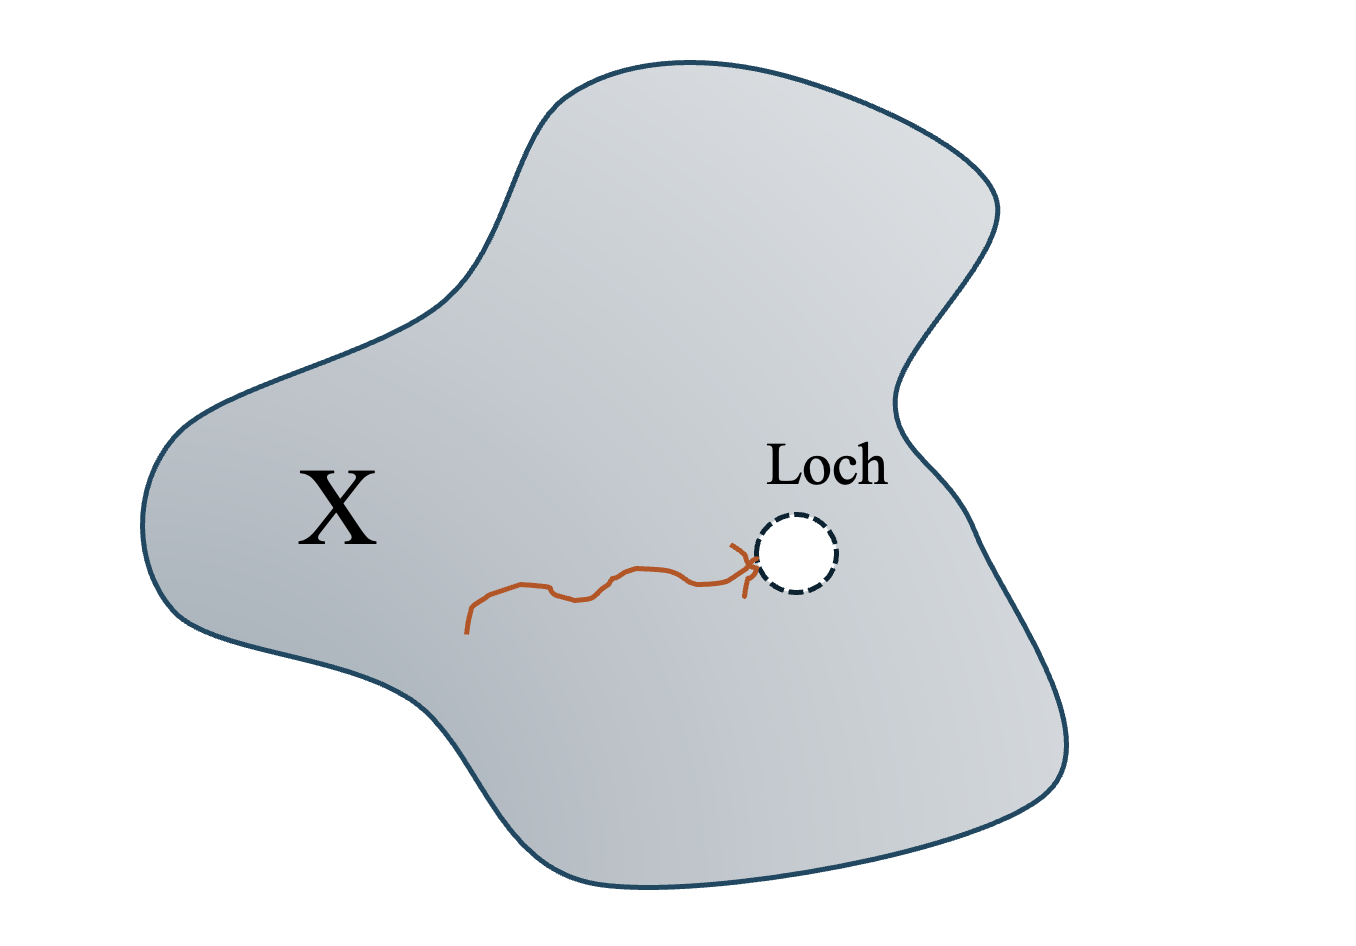
\includegraphics[width=0.64\linewidth]{docimgs/Kein_Hilbertraum.png}\\
        Kein Hilbertraum
        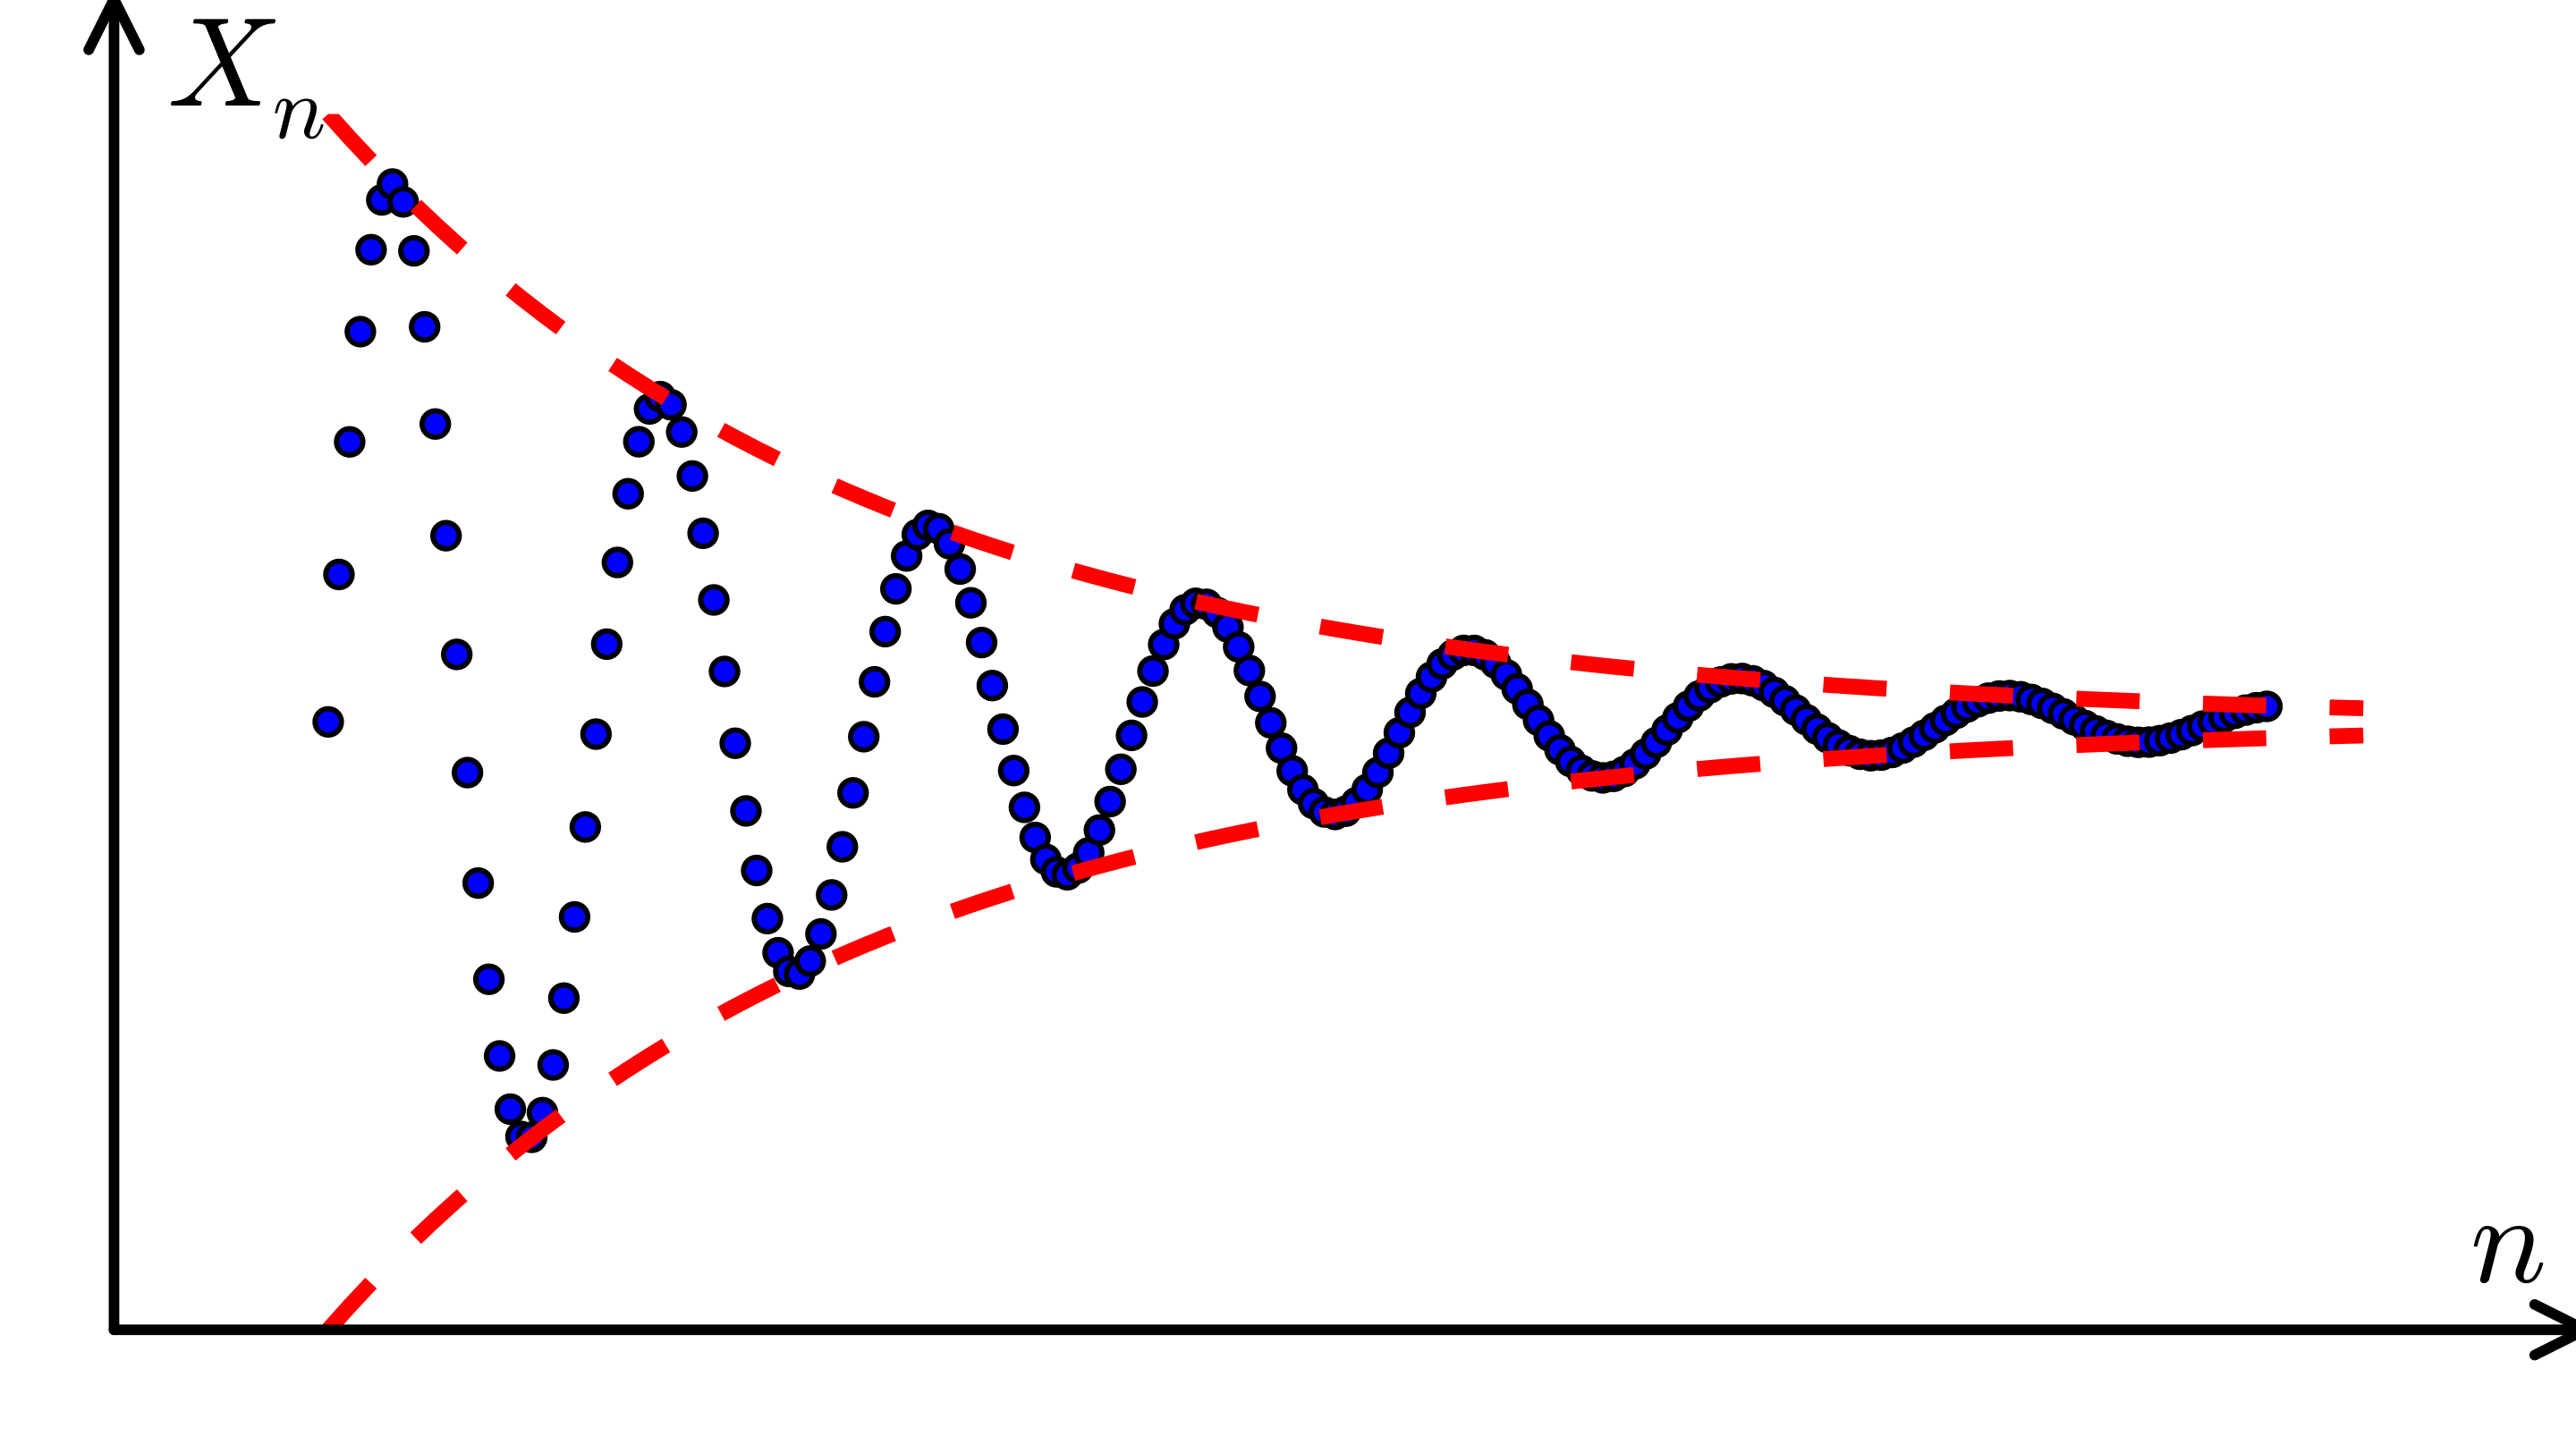
\includegraphics[width=0.8\linewidth]{docimgs/Cauchy_Folge.png}\\
        Cauchy-Folge
    \end{multicols}
\end{center}

\vspace*{-0.75cm}
\subsection*{Inneres Produkt (Skalarprodukt)}
\vspace*{-0.5cm}
\textbf{Definition:} Sei $X$ ein linearer Raum. Eine Abbildung $\langle \cdot, \cdot \rangle : X \times X \to \mathbb{C}$ von zwei Variablen in diesem Raum $X$ heisst inneres Produkt, wenn sie folgende Eigenschaften erfüllt:
\vspace*{-0.5cm}
\begin{itemize}
    \item[(i)] Additivität im 1. Argument: $\langle x + y, \; z\rangle = \langle x, \; z\rangle + \langle y, \; z\rangle$
    \item[(ii)] Homogenität im 1. Argument: $\langle \alpha x, \; y \rangle = \alpha \langle x, \; y \rangle$
    \item[(iii)] Konjugierte Symmetrie: $\langle x, \; y\rangle = \langle y, \; x\rangle^*$
    \item[(iv)] Positive Definitheit: $\langle x, \; x\rangle \geq 0$ und $\langle x, \; x\rangle = 0 \Leftrightarrow x = 0$
\end{itemize}

\vspace*{-0.75cm}
\begin{itemize}[leftmargin = 0pt]
    \begin{comment}
        \item[] \textbf{Beispiele für innere Produkte:}
    \begin{multicols}{2}
        \begin{itemize}
            \item[] $\langle x, \; y\rangle = \sum_{j=1}^d x_j y_j$ in $\mathbb{R}^d$
            \item[] $\langle f, \; g\rangle =\int_0^1 f(t)\overline{g(t)}dt$ in $L^2$
        \end{itemize}
    \end{multicols}
    \end{comment}
    \item[] \textbf{Bemerkungen:}\begin{itemize}
        \item Additiv im 2. Argument: $\langle x, \; y+z \rangle = \langle y + z, \; x \rangle^* = \langle y, \; x \rangle^* + \langle z, \; x \rangle^* = \langle x, \; y \rangle + \langle x, \; z \rangle$
        \item komplexe Konjugation: $\langle x, \; \alpha y\rangle = \langle \alpha y, \; x \rangle^* = \alpha^* \langle y, \; x \rangle^* = \alpha^* \langle x, \; y \rangle$
    \end{itemize}
\end{itemize}


\vspace*{-1cm}
\subsubsection*{Induzierte Norm}
\vspace*{-0.5cm}
Sei $X$ ein linearer Raum und $\langle \cdot, \cdot\rangle$ ein inneres Produkt auf $X \times X$. Dann ist $||x|| := \sqrt{\langle x, \; x\rangle}$ die von diesem Skalarprodukt \textbf{induzierte Norm}.

\pagebreak

\section*{Orthogonalität}
\vspace*{-0.5cm}
\begin{itemize}[leftmargin=0pt]
    \item[] \textbf{Definition:} Sei $x_1, x_2 \in X$, wobei $X$ ein linearer Raum mit Skalarprodukt $\langle \cdot, \cdot \rangle$ ist. $x_1$ und $x_2$ heissen \textbf{orthogonal} $(x_1 \perp x_2)$, falls $\langle x_1, \; x_2\rangle = 0$.
    \item[] \textbf{Bemerkung:} Orthogonale Vektoren sind linear unabhängig.
    \item[] \textbf{Bemerkung:} $n$ paarweise orthogonale Einheitsvektoren in einem linearen Raum der Dimension $n$ bilden eine orthonormale Basis in diesem Raum.
    \item[] \textbf{Satz des Pythagoras:}
    \item[] \fcolorbox{darkblue}{lightblue}{%
            \parbox{\dimexpr\linewidth-2\fboxsep-2\fboxrule\relax}{\centering Wenn $\langle x, \; y \rangle = 0$, \hspace{10pt}dann \hspace{10pt}$||x + y||^2 = ||x||^2 + ||y||^2$}}
    \item[] \textit{Beweis:} $||x+y||^2 = \langle x + y, \; x + y \rangle = \langle x, \; x + y \rangle + \langle y, \; x + y \rangle $ 
    \item[] \hspace{84pt} $= \underbrace{\langle x, \; x \rangle}_{||x||^2} + \underbrace{\langle x, \; y \rangle}_{0} + \underbrace{\langle y, \; x \rangle}_{\small{\langle x, \; y \rangle^* = 0}} + \underbrace{\langle y, \; y \rangle}_{||y||^2} = ||x||^2 + ||y||^2 \hspace{135pt} \blacksquare$
    \begin{comment}
        \item[] 
\begin{tikzpicture}
        % Define the box size and grid spacing
        \draw[step=0.5cm,gray!50,very thin] (0,0) grid (16.5,1.5); % (0,0) is bottom-left corner, (10,10) is top-right corner
        \end{tikzpicture}
    \end{comment}
    \item[] \textbf{Cauchy-Schwarz Ungleichung:}
    \item[] \fcolorbox{darkblue}{lightblue}{%
            \parbox{\dimexpr\linewidth-2\fboxsep-2\fboxrule\relax}{\centering $\left|\langle u, \; v \rangle \right| \leq ||u|| \cdot ||v|| $}}
    \item[] Intuition für $\mathbb{R}^2$: \hspace{10pt} $\left| \langle u, \; v \rangle \right| = ||u|| \cdot ||v|| \cdot \underbrace{\left| \cos \angle(u, \; v) \right|}_{\in [0,1]}$
\end{itemize}

\vspace*{-1.5cm}
\subsection*{Aufgabe 16}
\vspace*{-0.5cm}
Satz von Pythagoras: In der Vorlesung wird gezeigt, dass der Satz von Pythagoras für Signale $u_1, \; u_2 \in L^2$ wie folgt gilt: $\langle u_1, \; u_2 \rangle = 0$ impliziert $||u_1 + u_2||_2 = ||u_1||_2 + ||u_2||_2$. Beweisen Sie den allgemeinen Satz: Wenn das $n$-Tupel von Signalen $(u_1, \dots, u_n)$ in $L^2$ orthogonal ist, dann gilt
$$||u_1 + u_2 + \dots + u_n||^2 = ||u_1||^2 + ||u_2||^2 + \dots + ||u_n||^2$$.

\vspace*{-0.5cm}

\begin{tikzpicture}
    % Define the box size and grid spacing
    \draw[step=0.5cm,gray!50,very thin] (0,0) grid (16.5,7); % (0,0) is bottom-left corner, (10,10) is top-right corner
\end{tikzpicture}

\pagebreak

\subsection*{Vollständiges Orthonormalsystem}
\vspace*{-0.5cm}
\textbf{Definition:} Die Familie $\{e_l\}_{l = -\infty}^\infty$ von Vektoren in $X$ ist ein vollständiges Orthonormalsystem für den Hilbertraum $X$, wenn folgende Eigenschaften erfüllt sind.

\vspace*{-0.5cm}
\begin{enumerate}
    \item $\langle e_l, \; e_{l'} \rangle = \begin{cases}
        1, \hspace{12pt} l = l' \\
        0, \hspace{12pt} \text{sonst}
        \end{cases}$ \hspace{12pt}, für $l,l' \in \mathbb{Z}$
    \item Für jedes $x\in X$ gilt $||x||^2 = \displaystyle\sum_{l=-\infty}^\infty |\langle x, \; e_l \rangle|^2$
\end{enumerate}

\vspace*{-0.5cm}
Wenn $\{e_l\}_{l = -\infty}^\infty$ ein vollständiges Orthonormalsystem für $X$ ist, dann kann jedes $x\in X$ in der Form $x = \sum_{l=-\infty}^\infty \langle x, \; e_l \rangle e_l = \sum_{l=-\infty}^\infty c_l e_l$ dargestellt werden.

\subsection*{$L^2$ als unendlich dimensionaler normierter Raum}
\vspace*{-0.5cm}
Betrachte den linearen Unterraum $L^2([0,1])$ von $L^2$, also den linearen Raum der auf das Intervall $[0,1]$ beschränkten Signale, die quadratisch integrierbar sind:
$$L^2\left( [0,1] \right) = \left\{ x: [0,1] \to \mathbb{C} \left| \int_0^1 |x(t)|^2 < \infty \right. \right\}$$

\vspace*{-0.5cm}
Wir untersuchen diesen linearen Raum auf seine unendliche Dimension und auf das vollständige Orthonormalsystem $\{e^{2 \pi i n t}\}_{n = -\infty}^\infty$ in diesem Raum.


\vfill \null
\pagebreak

\subsection*{Gram-Schmidt Orthonormalisierungsverfahren}
\vspace*{-0.5cm}
Sei $V$ ein linearer Raum mit Basis $\{ w_i \}_{i=1}^n = \{ w_1, \dots, w_n \}$ und Skalarprodukt $\langle \cdot, \cdot \rangle$. Dann existiert eine ONB $\{v_i\}_{i=1}^n = \{v_1, \dots, v_n\}$ mit Span$\{v_1, \dots, v_j\} = $ Span$\{w_1, \dots, w_j\}$ für alle $j = 1, \dots, n$.

\fcolorbox{darkblue}{lightblue}{%
\parbox{\dimexpr\linewidth-2\fboxsep-2\fboxrule\relax}{\begin{itemize}
    \item[] \textbf{Algorithmus}
    \item[] Für $j = 1, \; 2, \dots, n$:
    \item[] \begin{itemize}
        \item[] $v_j' = w_j - \displaystyle\sum_{i=1}^{j-1} \frac{\langle v_i, \; w_j \rangle }{\langle v_i, \; v_i \rangle} v_i$
        \item[] $v_j = \displaystyle\frac{v_j'}{||v_j'||}$
        \item[] $j \to j + 1$
    \end{itemize}
\end{itemize}}}

Die ersten drei Terme sehen wie folgt aus: (\textbf{Normierung nicht vergessen!})
\begin{multicols}{3}
    \begin{itemize}[leftmargin = 0pt]
        \item[] $v_1' = w_1$
        \item[] $v_2' = w_2 - \frac{\langle v_1, \; w_2 \rangle}{\langle v_1, \; v_1 \rangle} v_1$
        \item[] $v_3' = w_3 - \frac{\langle v_1, \; w_3 \rangle}{\langle v_1, \; v_1 \rangle} v_1 - \frac{\langle v_2, \; w_3 \rangle}{\langle v_2, \; v_2 \rangle} v_2$
    \end{itemize}
\end{multicols}

\vspace*{-0.5cm}
\subsection*{Aufgabe 18}
\vspace*{-0.5cm}
Es sei $X = \{x(t)=\alpha_0 + \alpha_1 t | t \in [0,1], \alpha_0,\alpha_1 \in \mathbb{R}\}$ der Raum aller reellen Polynome vom Grad $\leq 1$ auf dem Intervall $[0,1]$. Wir definieren das innere Produkt auf $X$ durch 
$$\langle x_1, \; x_2 \rangle = \displaystyle\int_0^1 x_1(t)x_2(t)\text{d}t, \hspace{12pt} x_1, x_2 \in X$$

%\vspace*{-0.5cm}
\begin{itemize}
    \item[a)] Gegeben seien $y_1(t) = 1 \in X$ und $y_2(t) = t \in X$. Bestimmen Sie den Kosinus des Winkels $\varphi$ zwischen $y_1(t)$ und $y_2(t)$, d.h., berechnen Sie $\cos (\varphi) = \frac{\langle y_1, \; y_2 \rangle}{||y_1|| \; ||y_2||}$.
    \item[] Stehen die Polynome $y_1(t)$ und $y_2(t)$ bezüglich dieses Skalarproduktes senkrecht aufeinander?
\end{itemize}



\begin{tikzpicture}
    % Define the box size and grid spacing
    \draw[step=0.5cm,gray!50,very thin] (0,0) grid (16.5,4.5); % (0,0) is bottom-left corner, (10,10) is top-right corner
\end{tikzpicture}


\pagebreak

\begin{itemize}
    \item[b)] Bestimmen Sie eine Orthonormalbasis von $X$ bezüglich des Skalarproduktes aus Aufgabe a).
\end{itemize}

\begin{tikzpicture}
    % Define the box size and grid spacing
    \draw[step=0.5cm,gray!50,very thin] (0,0) grid (16.5,16); % (0,0) is bottom-left corner, (10,10) is top-right corner
\end{tikzpicture}

\vfill \null
\pagebreak

\section*{Systeme und Systemeigenschaften}
\vspace*{-0.5cm}
\hspace{-0.3cm}

\includegraphics[width=0.95\linewidth]{docimgs/System_Blockschaltbild.png}

\textbf{Definition:} Ein System $H$ ist eine Abbildung, die einem Eingangssignal $x$ ein Ausgangssignal $y$ zuordnet. Man schreibt $y = Hx$

\subsection*{Linearität}
\vspace*{-0.5cm}
\textbf{Definition:} Ein System $H:X \to Y$ ist linear, wenn 
\vspace*{-0.5cm}
\begin{itemize}
    \item[(i)] Additivität: $H(x_1 + x_2) = Hx_1 + Hx_2$, für alle $x_1,x_2 \in X$
    \item[(ii)] Homogenität: $H(\alpha x) = \alpha H x$, für alle $x\in X$ und alle $\alpha \in \mathbb{C}$
\end{itemize}
\textbf{Bemerkungen:}
\vspace*{-0.5cm}
\begin{itemize}
    \item Ein System, das mindestens eine dieser beiden Bedingungen nicht erfüllt, heisst \textbf{nichtlinear}.
    \item Wenn $H$ ein lineares System ist, dann muss immer gelten: $H0 = 0$. Wenn dies also nicht erfüllt ist, dann muss $H$ nichtlinear sein.
\end{itemize}


\subsection*{Aufgabe 23}
\vspace*{-0.5cm}
Überprüfen Sie die folgenden Systeme auf Linearität.
\begin{multicols}{3}
    \begin{itemize}
        \item[a)] $(Hx)(t) = |x(t)|$
        \item[b)] $(Hx)(t) = x(t-1)+tx(t)$
        \item[c)] $(Hx)(t) = x(2)x(3)$
    \end{itemize}
\end{multicols}



\begin{tikzpicture}
    % Define the box size and grid spacing
    \draw[step=0.5cm,gray!50,very thin] (0,0) grid (16.5,4); % (0,0) is bottom-left corner, (10,10) is top-right corner
\end{tikzpicture}

\pagebreak


\begin{tikzpicture}
    % Define the box size and grid spacing
    \draw[step=0.5cm,gray!50,very thin] (0,0) grid (16.5,8); % (0,0) is bottom-left corner, (10,10) is top-right corner
\end{tikzpicture}

\subsection*{Aufgabe 24}
\vspace*{-0.5cm}
Es sei ein lineares System $H$ gegeben, welches auf die Eingangssignale $x_1(t)$ und $x_2(t)$ mit den Ausgangssignalen $y_1(t) = (Hx_1)(t) = 2 \sin (t)/t$ und $y_2(t) = (Hx_2)(t) = i e^{-t^2}$ antwortet. Finden Sie die Antwort des Systems H auf das Eingangssignal $x_3(t)$.
\vspace*{-0.5cm}
\begin{center}
    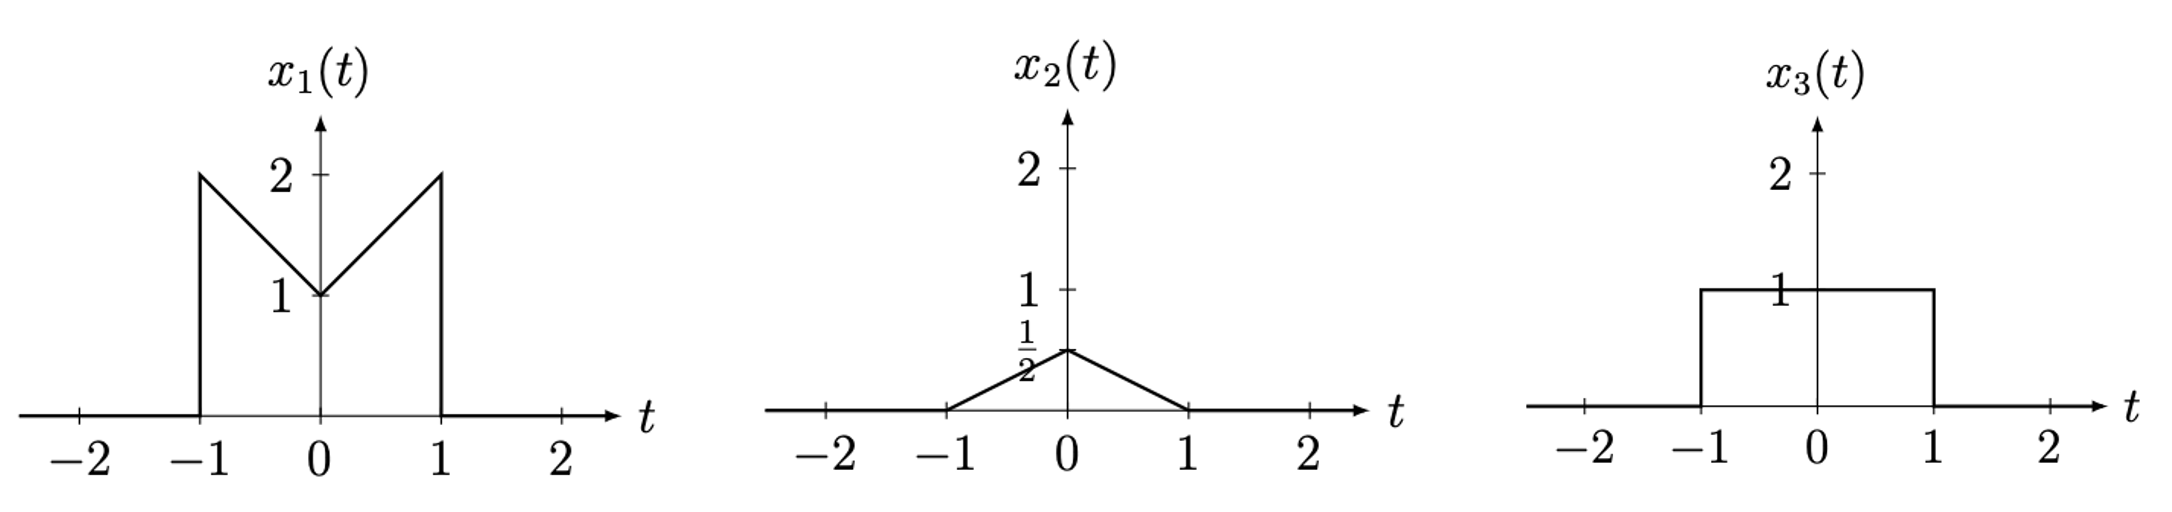
\includegraphics[width=\linewidth]{docimgs/Aufgabe_24_signale.png}
\end{center}

\begin{tikzpicture}
    % Define the box size and grid spacing
    \draw[step=0.5cm,gray!50,very thin] (0,0) grid (16.5,4); % (0,0) is bottom-left corner, (10,10) is top-right corner
\end{tikzpicture}


\vfill \null
\pagebreak

\subsection*{Nullraum}
\vspace*{-0.5cm}
\begin{itemize}[leftmargin = 0pt]
    \item[] \textbf{Definition:} Der Nullraum $\mathcal{N}(H)$ des linearen Systems $H:X \to Y$ ist die Teilmenge von $X$ definiert durch $\mathcal{N}(H) = \{x \in X : Hx = 0\}$.
    \item[] \textbf{Bemerkung:} $\mathcal{N}(H)$ ist ein linearer Unterraum von $X$.
\end{itemize}

\subsection*{Bildraum}
\vspace*{-0.5cm}
\begin{itemize}[leftmargin = 0pt]
    \item[] \textbf{Definition:} Der Bildraum $\mathcal{R}(H)$ des linearen Systems $H:X \to Y$ ist die Teilmenge von $Y$ definiert durch $\mathcal{R}(H) = \{y =Hx : x \in X\}$.
    \item[] \textbf{Bemerkung:} $\mathcal{R}(H)$ ist ein linearer Unterraum von $Y$.
\end{itemize}

\begin{center}
    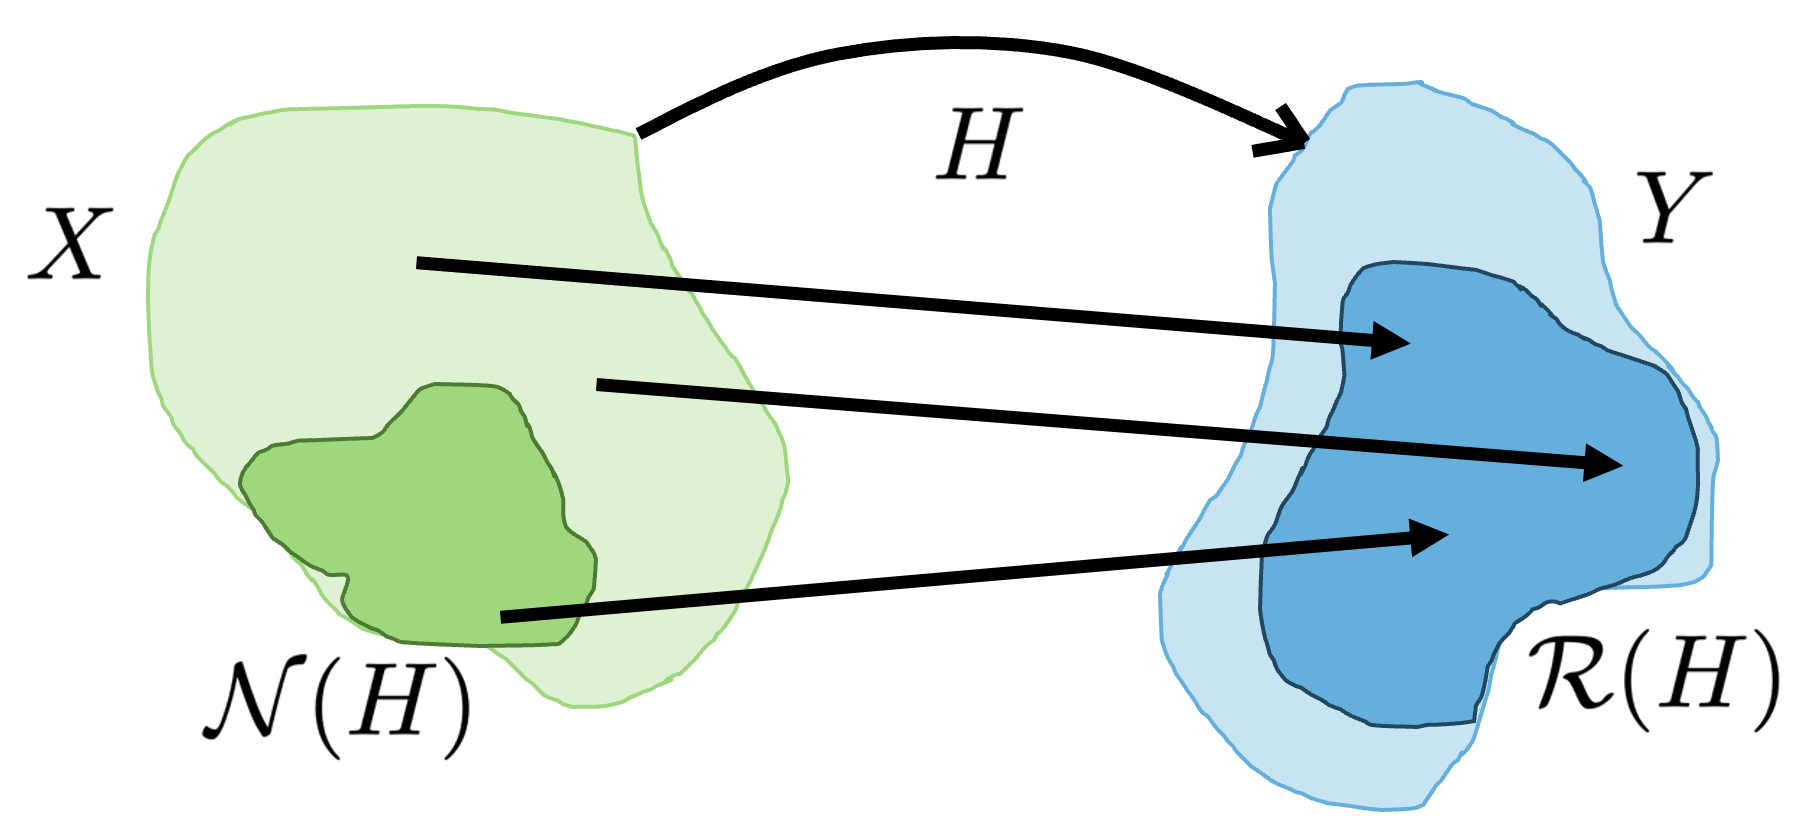
\includegraphics[width = 0.7\linewidth]{docimgs/Bildraum_Nullraum.png}
\end{center}


\subsection*{Stetigkeit}
\vspace*{-0.5cm}
\begin{itemize}[leftmargin = 0pt]
    \item[] \textbf{Theorem:} (\textit{Stetige Systeme}). Das System $H$ ist linear und stetig, dann und nur dann, wenn für jede konvergente Reihe $\sum_{i=1}^\infty \alpha_i x_i$ gilt:
    $$H\left( \sum_{i=1}^\infty \alpha_i x_i \right) = \sum_{i=1}^\infty \alpha_i H x_i$$
    \item[] \textbf{$\varepsilon-\delta$ Stetigkeit} (vgl. Analysis $1 \& 2$).\\Seien $(X, ||\cdot||)$ und $(Y, ||\cdot||)$ normierte lineare Räume. Dann heisst das System $H:X \to Y$ stetig in $x_0 \in X$, falls es zu jedem $\varepsilon > 0$ ein nur von $\varepsilon$ abhängiges $\delta >0$ gibt, so dass für alle $x\in X$ mit $||x-x_0||<\delta$ folgt, dass $||Hx-Hx_0||\leq \varepsilon$.
    \item[] \textbf{Bemerkung:} Ab hier nehmen wir in SST1 immer an, dass ein lineares Sysem auch stetig ist, sodass die Gleichung in obigem Theorem immer gilt.
\end{itemize}


\end{document}